\documentclass[a4paper,11pt,fleqn,twoside,openright]{memoir} % Brug openright hvis chapters skal starte på højresider; openany, oneside

%%%% PACKAGES %%%%

%  Oversættelse og tegnsætning  %
\usepackage[utf8]{inputenc}					% Gør det muligt at bruge æ, ø og å i sine .tex-filer

\raggedbottom
\usepackage[all]{nowidow}
\usepackage[T1]{fontenc}  % Hjælper med orddeling ved æ, ø og å. Sætter fontene til at være ps-fonte, i stedet for bmp	
\usepackage{syntax}
\usepackage{everyshi}
\makeatletter
\let\totalpages\relax
\newcounter{mypage}
\EveryShipout{\stepcounter{mypage}}
\AtEndDocument{\clearpage
   \immediate\write\@auxout{%
    \string\gdef\string\totalpages{\themypage}}}
\makeatother
\usepackage{longtable}
\usepackage{lscape}
\usepackage[lined,boxed,linesnumbered]{algorithm2e}
\usepackage{latexsym}										% LaTeX symboler
\usepackage{xcolor,ragged2e,fix-cm}			% Justering af elementer
\usepackage{pdfpages} % Gør det muligt at inkludere pdf-dokumenter med kommandoen \includepdf[pages={x-y}]{fil.pdf}	
\usepackage{fixltx2e}					% Retter forskellige bugs i LaTeX-kernen
\usepackage{color}
\definecolor{darkgray}{rgb}{0.95,0.95,0.95}
\usepackage{listings}
\usepackage{tikz}
\usepackage{qtree}


 \lstloadlanguages{% Check Dokumentation for further languages ...
         %[Visual]Basic
         %Pascal
         C
	%[Sharp]C
         %C++
         %XML
         %HTML
        % Java
 }
\lstset{ %
inputencoding=utf8,
literate=%
{æ}{{\ae}}1
{å}{{\aa}}1
{ø}{{\o}}1
{Æ}{{\AE}}1
{Å}{{\AA}}1
{Ø}{{\O}}1,
language=[Sharp]C,                % the language of the code
basicstyle=\footnotesize\ttfamily,       % the size of the fonts that are used for the code
float = H,
xleftmargin = 10pt,
xrightmargin = 10pt,
rulecolor = \color{black},
numbers=left,                   % where to put the line-numbers
numberstyle=\footnotesize,      % the size of the fonts that are used for the line-numbers
stepnumber=1,                   % the step between two line-numbers. If it's 1, each line 
                                % will be numbered
numbersep=5pt,                  % how far the line-numbers are from the code
showspaces=false,               % show spaces adding particular underscores
showstringspaces=false,         % underline spaces within strings
showtabs=false,                 % show tabs within strings adding particular underscores
tabsize=2,                      % sets default tabsize to 2 spaces
captionpos=b,                   % sets the caption-position to bottom
breaklines=true,                % sets automatic line breaking
breakatwhitespace=false,        % sets if automatic breaks should only happen at whitespace
               % show the filename of files included with \lstinputlisting;
                                % also try caption instead of title
escapeinside={\%*}{*)},         % if you want to add a comment within your code
keywordstyle=\color[rgb]{0,0,1},
commentstyle=\color[rgb]{0.133,0.545,0.133},
stringstyle=\color[rgb]{0.627,0.126,0.941},
morekeywords={begin, function, end, nothing, bool, string, OR, AND, using, from, to, step, container, HIGH, LOW}
}

% add frame environment
\usepackage[%
    style=1,
    skipbelow=\topskip,
    skipabove=\topskip
]{mdframed}
\mdfsetup{%
    leftmargin=0pt,
    rightmargin=0pt,
    backgroundcolor=darkgray,
    middlelinecolor=black,
    roundcorner=10
}

% needed for \lstcapt
\def\ifempty#1{\def\temparg{#1}\ifx\temparg\empty}

% make new caption command for listings
\usepackage{caption}
\newcommand{\lstcapt}[2][]{%
    \ifempty{#1}%
        \captionof{lstlisting}{#2}%
    \else%
        \captionof{lstlisting}[#1]{#2}%
    \fi%
    \vspace{0.75\baselineskip}%
}

\usepackage{tabularx}
\usepackage{changepage}

																			
%  Figurer og tabeller floats %
\pdfoptionpdfminorversion=6	% Muliggør inkludering af pdf dokumenter, af version 1.6 og højere
\usepackage{graphicx} 		% Pakke til jpeg/png billeder
\usepackage{rotating}	

%  Matematiske formler og maskinkode 
\usepackage{amsmath,amssymb,stmaryrd} 	% Bedre matematik og ekstra fonte
\usepackage{textcomp}                 	% Adgang til tekstsymboler
\usepackage{mathtools}			% Udvidelse af amsmath-pakken.
\usepackage{siunitx}			% Flot og konsistent præsentation af tal og enheder med \SI{tal}{enhed}

%  Referencer, bibtex og url'er  %
\usepackage{url}	% Til at sætte urler op med. Virker sammen med ref
%\usepackage[danish]{varioref} % Giver flere bedre mulighed for at lave krydshenvisninger
\usepackage[english]{varioref} % Giver flere bedre mulighed for at lave krydshenvisninger
\usepackage{natbib}	% Litteraturliste med forfatter-år og nummerede referencer
\usepackage{xr}		% Referencer til eksternt dokument med \externaldocument{<NAVN>}
\usepackage{nomencl}	% Pakke til at danne nomenklaturliste
\makenomenclature		% Nomenklaturliste

%  Floats  %
\let\newfloat\relax 	% Memoir har allerede defineret denne, men det gør float pakken også
\usepackage{float}
%\usepackage[footnote,draft,danish,silent,nomargin]{fixme}	% Indsæt rettelser og lignende med \fixme{...} Med final i stedet for draft, udløses en error for hver fixme, der ikke er slettet, når rapporten bygges.
\usepackage[draft,silent]{fixme}

%%%% CUSTOM SETTINGS %%%%

%  Marginer  %
\setlrmarginsandblock{3.5cm}{2.5cm}{*}	% \setlrmarginsandblock{Indbinding}{Kant}{Ratio}
\setulmarginsandblock{2.5cm}{3.0cm}{*}	% \setulmarginsandblock{Top}{Bund}{Ratio}
\checkandfixthelayout 

%  Litteraturlisten  %
\bibpunct[,]{[}{]}{;}{a}{,}{,} 	% Definerer de 6 parametre ved Harvard henvisning (bl.a. parantestype og seperatortegn)
\bibliographystyle{bibtex/harvard}	% Udseende af litteraturlisten. Ligner dk-apali - mvh Klein

%  Indholdsfortegnelse  %
\setsecnumdepth{subsubsection}	% Dybden af nummerede overkrifter (part/chapter/section/subsection)
\maxsecnumdepth{subsubsection}	% Ændring af dokumentklassens grænse for nummereringsdybde
\settocdepth{subsection} 		% Dybden af indholdsfortegnelsen


%  Visuelle referencer  %
\usepackage[colorlinks, bookmarksnumbered, bookmarksdepth=4]{hyperref} % Giver mulighed for at ens referencer bliver til klikbare hyperlinks. .. [colorlinks]{..}
%\usepackage{memhfixc}
\hypersetup{pdfborder = 0 0 0}	% Fjerner ramme omkring links i fx indholsfotegnelsen og ved kildehenvisninger 
\hypersetup{			%	Opsætning af farvede hyperlinks
    colorlinks = false,
    linkcolor = black,
    anchorcolor = black,
    citecolor = black
}

\definecolor{gray}{gray}{0.80}					% Definerer farven grå

%  Kapiteludssende  %
\definecolor{numbercolor}{gray}{0.7}			% Definerer en farve til brug til kapiteludseende
\newif\ifchapternonum

\makechapterstyle{jenor}{			% Definerer kapiteludseende -->
  \renewcommand\printchaptername{}
  \renewcommand\printchapternum{}
  \renewcommand\printchapternonum{\chapternonumtrue}
  \renewcommand\chaptitlefont{\fontfamily{pbk}\fontseries{db}\fontshape{n}\fontsize{25}{35}\selectfont\raggedleft}
  \renewcommand\chapnumfont{\fontfamily{pbk}\fontseries{m}\fontshape{n}\fontsize{1in}{0in}\selectfont\color{numbercolor}}
  \renewcommand\printchaptertitle[1]{%
    \noindent
    \ifchapternonum
    \begin{tabularx}{\textwidth}{X}
    {\let\\\newline\chaptitlefont ##1\par} 
    \end{tabularx}
    \par\vskip-2.5mm\hrule
    \else
    \begin{tabularx}{\textwidth}{Xl}
    {\parbox[b]{\linewidth}{\chaptitlefont ##1}} & \raisebox{-15pt}{\chapnumfont \thechapter}
    \end{tabularx}
    \par\vskip2mm\hrule
    \fi
  }
}			% <--

\chapterstyle{jenor}	% Valg af kapiteludseende - dette kan udskiftes efter ønske
\usepackage{wrapfig}


%\renewcommand{\headrulewidth}{0.4pt}
%\renewcommand{\footrulewidth}{0.4pt}

\usepackage{enumitem}
% Sidehoved %

\makepagestyle{custom} % Definerer sidehoved og sidefod - kan modificeres efter ønske -->
\makepsmarks{custom}{																						
\def\chaptermark##1{\markboth{\itshape\thechapter. ##1}{}} % Henter kapitlet den pågældende side hører under med kommandoen \leftmark. \itshape gør teksten kursiv
\def\sectionmark##1{\markright{\thesection. ##1}{}}	% Henter afsnittet den pågældende side hører under med kommandoen \rightmark
} % Sidetallet skrives med kommandoen \thepage	
\makeevenhead{custom}{\leftmark}{P4, Aalborg University}{Group SW407F13} % Definerer lige siders sidehoved efter modellen \makeevenhead{Navn}{Venstre}{Center}{Højre}
\makeoddhead{custom}{Group SW407F13}{P4, Aalborg University}{\leftmark} % Definerer ulige siders sidehoved efter modellen \makeoddhead{Navn}{Venstre}{Center}{Højre}

\usepackage{lastpage}
\usepackage{ifthen}
\usepackage{intcalc}
\usepackage{nth}

\makeevenfoot{custom}{Side \thepage}{}{}	% Definerer lige siders sidefod efter modellen \makeevenfoot{Navn}{Venstre}{Center}{Højre}
\makeoddfoot{custom}{}{}{Side \thepage}% Definerer ulige siders sidefod efter modellen \makeoddfoot{Navn}{Venstre}{Center}{Højre}		
\makeheadrule{custom}{\textwidth}{0.5pt}	 % Tilføjer en streg under sidehovedets indhold
\makefootrule{custom}{\textwidth}{0.5pt}{1mm}	% Tilføjer en streg under sidefodens indhold

\copypagestyle{nychapter}{custom} % Følgende linier sørger for, at sidefoden bibeholdes på kapitlets første side
\makeoddhead{nychapter}{Group SW407F13, Aalborg Universitet}{P4}{\leftmark}
\makeevenhead{nychapter}{Group SW407F13, Aalborg Universitet}{P4}{\leftmark}
\makeheadrule{nychapter}{\textwidth}{0pt}
\aliaspagestyle{chapter}{nychapter}	% <--
\aliaspagestyle{cleared}{custom}

\pagestyle{custom}

%%%% CUSTOM COMMANDS %%%%

% Billede hack %
\newcommand{\figur}[4]{
		\begin{figure}[H] \centering
			\includegraphics[width=#1\textwidth]{billeder/#2}
			\caption{#3}\label{#4}
		\end{figure} 
}

% højrepil %
\newcommand{\ra}[0]{\rightarrow}
% epsilon %
\newcommand{\eps}{\varepsilon}

% Vektor hack %
\newcommand{\vektor}[3]{
			$\begin{pmatrix}
				#1 \\ #2 \\ #3
			\end{pmatrix}$
}

%kode
\newcommand{\kode}[3]{
\noindent
\begin{minipage}{\textwidth}
\begin{mdframed}
		\lstinputlisting{kode/#3}

\end{mdframed}\lstcapt{#1}\label{lst:#2}
\end{minipage}
}

\newenvironment{code}[2]
{\def\fooNoI{#1} \def\fooNoII{#2}\noindent \begin{minipage}{\textwidth}\begin{mdframed}}{\end{mdframed}\lstcapt{\fooNoII}\label{lst:\fooNoI}\end{minipage}}

% quotering
\newcommand{\gaas}[{1}]{``#1''}

% lilleitem
%\newenvironment{noindlist}
 %{\vspace{-5mm}\begin{list}{\labelitemi}{\leftmargin=1em \itemindent=0em }
%\addtolength{\itemsep}{-0.5\baselineskip}}
 %{\end{list}
%\vspace{-20em}}

\newenvironment{noindlist}
 {\vspace{-5mm}\begin{list}{\labelitemi}{\leftmargin=1em \itemindent=0em }
        \setlength{\topsep}{0pt}
        \setlength{\parskip}{0pt}
        \setlength{\partopsep}{0pt}
        \setlength{\parsep}{0pt}         
        \setlength{\itemsep}{0pt} }
 {\end{list}}

\newcommand{\doublesignaturestart}[2]{%
  \parbox{\textwidth}{
    \centering Aalborg \today\\
    \vspace{2cm}

    \parbox{7cm}{
      \centering
      \rule{6cm}{1pt}\\
       #1 
    }
    \hfill
    \parbox{7cm}{
      \centering
      \rule{6cm}{1pt}\\
      #2
    }
  }
}

\newcommand{\longtablesetting}[1]{
\endhead
\multicolumn{#1}{c}{\textit{Continued on the next page}} \\
\endfoot
\endlastfoot
}

\newcommand{\subsubsubsection}[1]{
\textbf{#1}
}

\newcommand{\doublesignature}[2]{%
  \parbox{\textwidth}{
\vspace{2cm}
    \parbox{7cm}{
      \centering
      \rule{6cm}{1pt}\\
       #1 
    }
    \hfill
    \parbox{7cm}{
      \centering
      \rule{6cm}{1pt}\\
      #2
    }
  }
}


%%%% ORDDELING %%%%

\hyphenation{hvad hvem hvor}
\newcolumntype{R}{>{\raggedright\arraybackslash}X}

%----------------SPROG------------------------
%----------------dk
%\usepackage[danish]{babel}							% Dansk sporg, f.eks. tabel, figur og kapitel
%\renewcommand{\algorithmcfname}{Algoritme}
%\renewcommand*{\lstlistingname}{Kodeudsnit}
%----------------en
\usepackage[english]{babel}

\begin{document}	% Starter dokumentet - obligatorisk

\frontmatter % Forindhold - nummereres med romertal

\thispagestyle{empty}
\begin{flushright}
\vspace{3cm}

\phantom{hul}

\phantom{hul}

\phantom{hul}

\textsl{P4 Project} \\ \vspace{1cm}

\rule{0.8\textwidth}{3mm} \\ \vspace{1.5cm}
%\vspace{1cm}

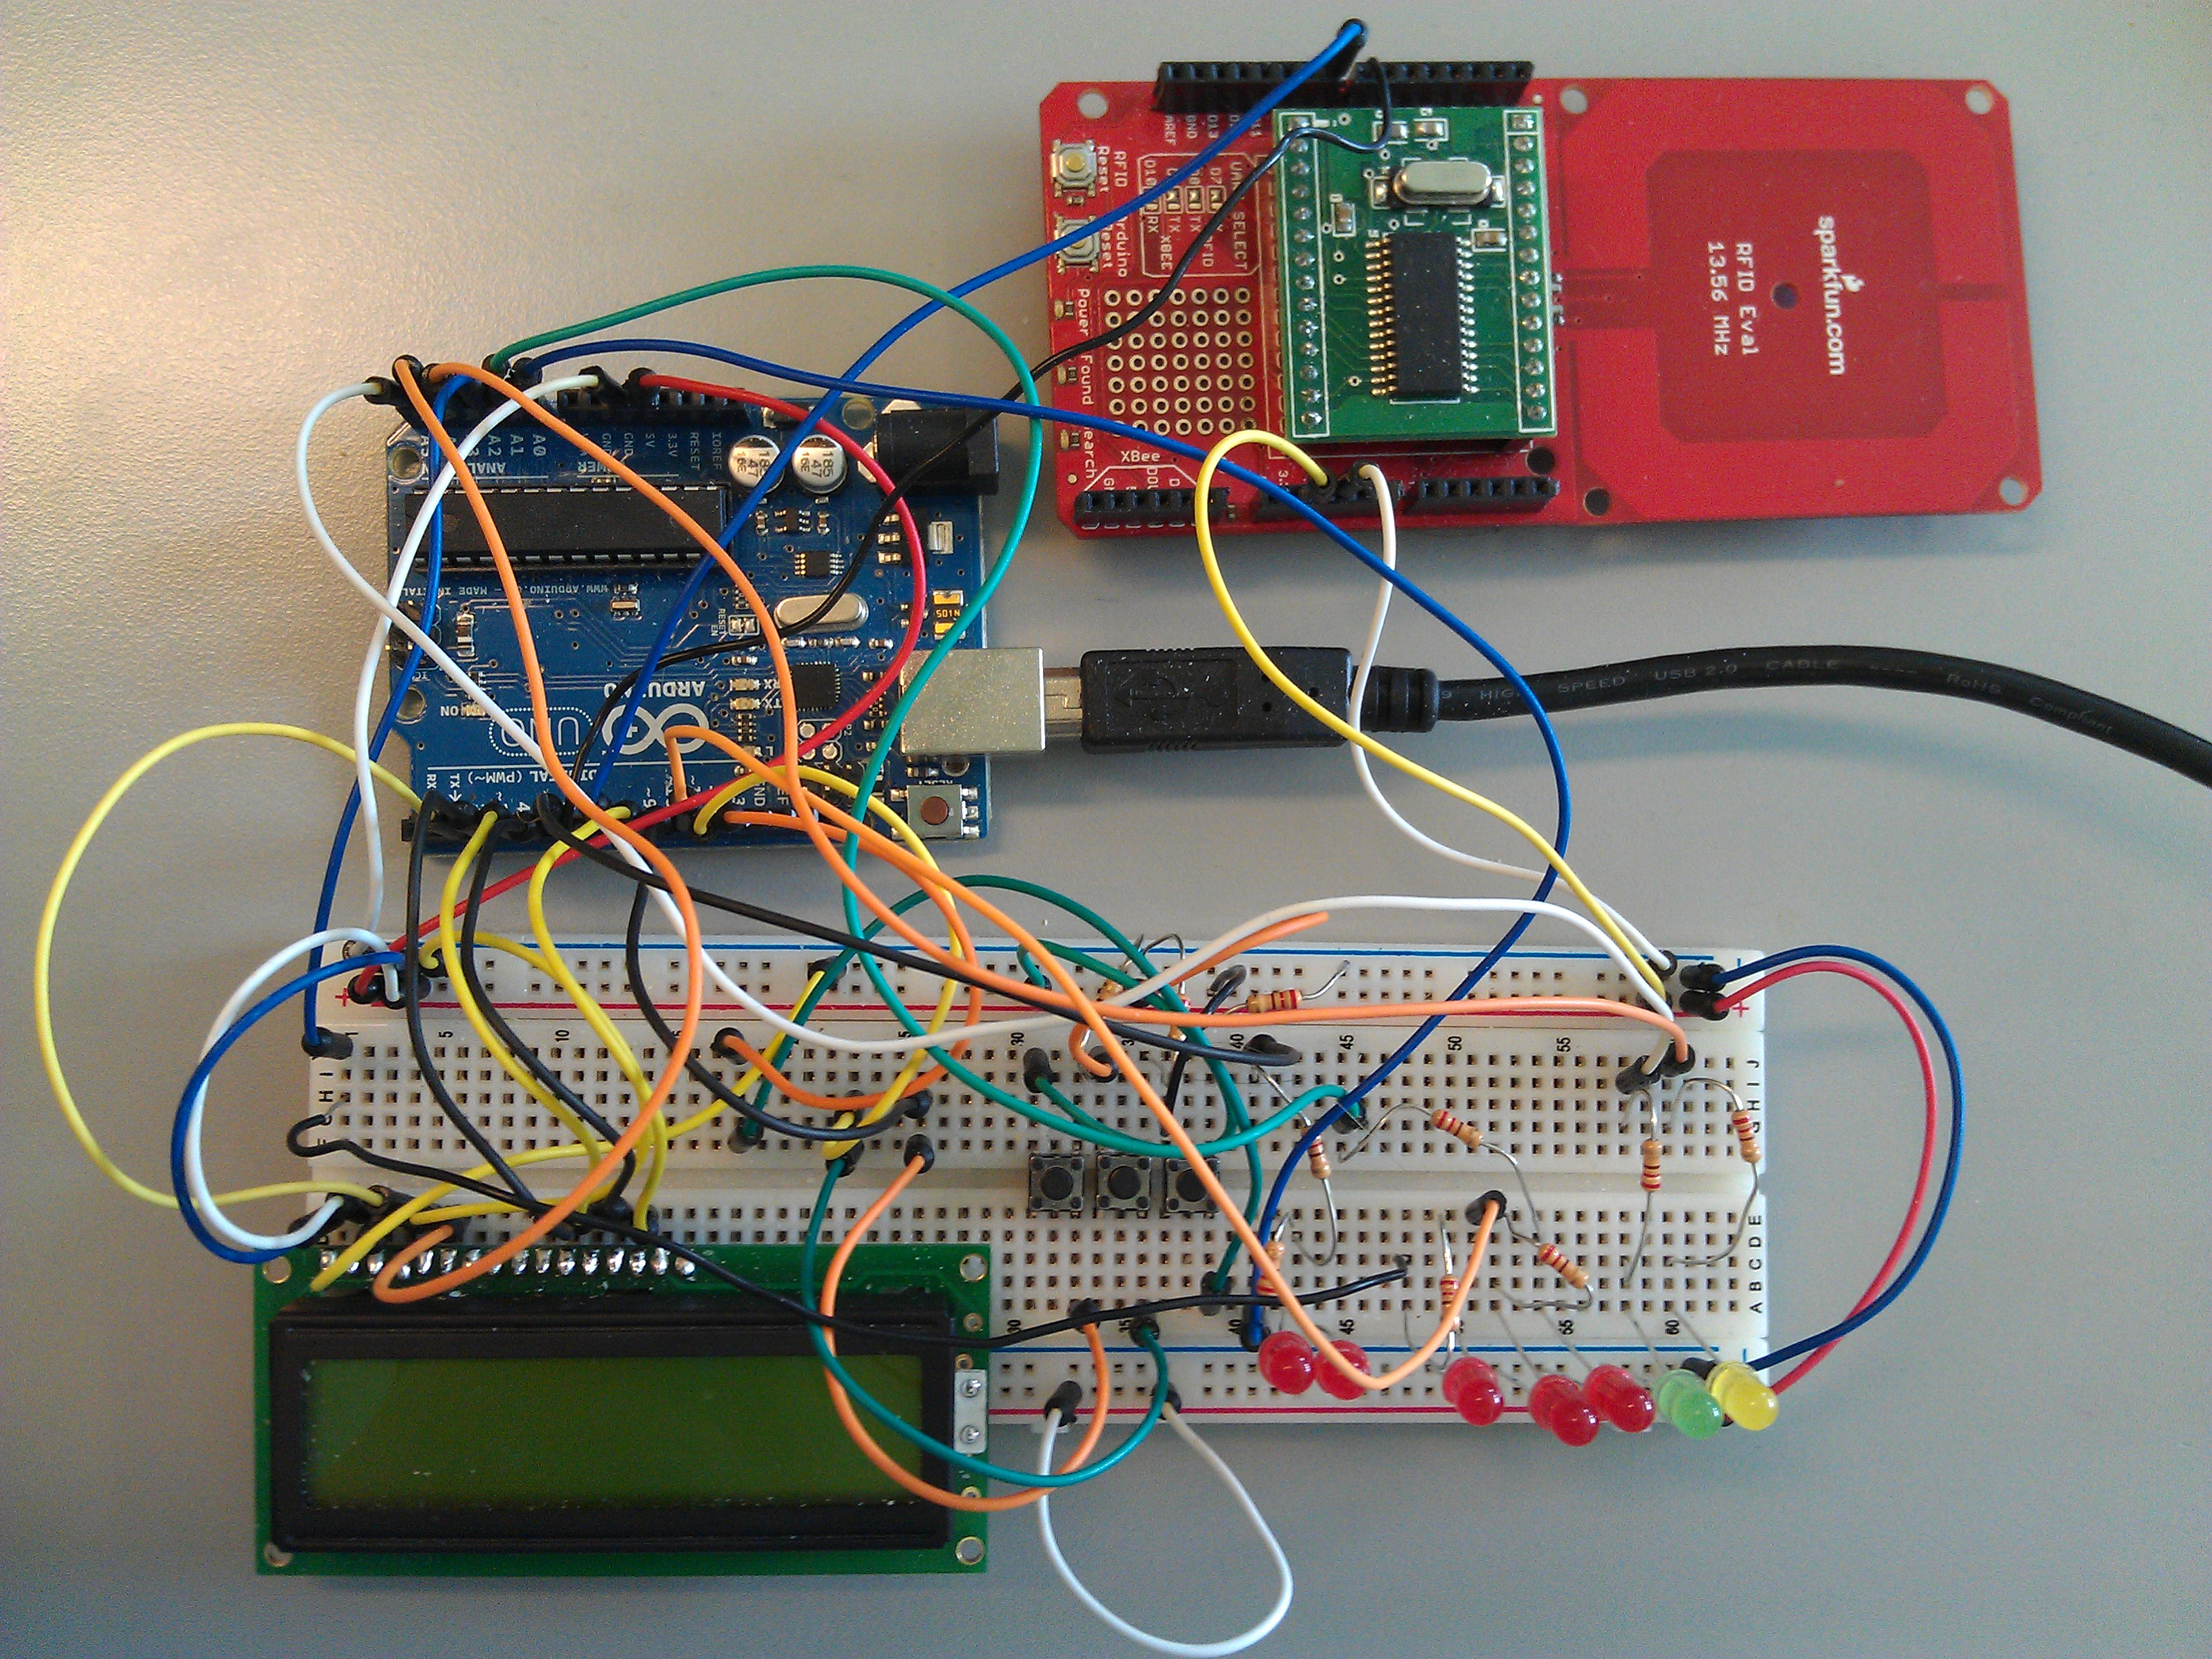
\includegraphics[width=0.8\textwidth]{billeder/HardwareSetup.png}

\vspace{1.5cm} 
\textsc{\Large SPLAD \\
P4 projekt\\
Group SW407F13\\
Software\\
Department of Computer Science\\
Aalborg University\\
May 2013\\
~\\
}

\includegraphics[width=0.35\textwidth]{billeder/AAUUKSTUDENTREPORTbluergb.png}
\end{flushright}

\cleardoublepage % Indsætter tom side (hvis nødvendigt)

% Dette er LaTeX-versionen af titelbladet for tek-nat-basis-rapporter 2004 efterår
% Filen kræver:
% Universitetets logo:  aau-logo.png (for LaTeX) eller aau-logo.ps (for LaTeX)
% Synopsis: En fil ved navn synopsis.tex

% Udarbejdet af: Hans Hüttel (hans@cs.auc.dk) 21. maj 2003
% Rettet af Morten Christophersen (mortench@tnb.aau.dk) 30. nov 2004(ændret til nyt design 2004 efterår)

%\documentclass[11pt]{article}
%\ifx\pdfoutput\undefined 
%\usepackage[dvips]{graphicx}
%\else
%\usepackage[pdftex]{graphicx} 
%\usepackage{type1cm} \fi
  %  \usepackage[ansinew]{inputenc}
    %\usepackage{a4}

%\begin{document} 
%\thispagestyle{empty}
%\begin{titlepage}

\begin{nopagebreak}
{\samepage
\hspace{8cm}
\begin{tabular}{r}
\parbox{\textwidth}{  \raisebox{11mm}{ 
\includegraphics[height=4cm]{billeder/AAUUKSTUDENTREPORTbluergb.png}}
\hfill
\\
\parbox{8cm}{\begin{tabular}{l}
{\small \textbf{Department of Computer Science}}\\
{\small Selma Lagerlöfs Vej 300} \\
{\small DK-9220 Aalborg East} \\
{\small http://www.cs.aau.dk/en}
\end{tabular}}}

\end{tabular}
\hspace{0cm}

\vspace{-5cm}
\begin{tabular}{cc}
\parbox{7cm}{
\begin{description}

\item {Titel:} 

SPLAT - Special Programming Language for Arduino Tipple-mixer

\end{description}

\parbox{8cm}{

\begin{description}
\item {Project period:}\\
   P4, spring 2012\\
  \hspace{4cm}
\item { Project group:}\\
  SW407F13\\
  \hspace{4cm}
\item { Group members:}\\
Aleksander Sørensen Nilsson \\
Christian Jødal O'Keeffe \\
Kasper Plejdrup\\
Mette Thomsen Pedersen \\
Niels Brøndum Pedersen \\
Rasmus Fischer Gadensgaard \\
  \hspace{2cm}
\item { Supervisor:}\\
Ricardo Gomes Lage\\
\end{description}
}
\begin{description}
\item { Total number of pages: }\\ \totalpages
\item { Project end: }\\
$29^{\text{th}}$ of May, 2013
\end{description}

\vfill } &
\parbox{7cm}{
  \vspace{.15cm}
  \hfill \\ \\
  \begin{tabular}{l}
  { Synopsis:}\\%\bigskip 
  \fbox{
    \parbox{6.5cm}{\bigskip
     {\vfill{\small This report starts off with a description of an environment where drinks are an essential part, this leads to the following problem statement:
"How can a programming language be developed, which makes it suitable for the hobbyist programmer to program drinks machines based on Arduino platforms?"
The product of this project is a programming language with a compiler which can make it easier to program a machine which can mix and serve drinks. The syntax of the program language is written in BNF and the compiler is developed using the parser and lexer generator ANTLR. Lastly, unit testing is used to test certain parts of the compiler to see if they work as intended. It has been concluded that this project gives a fulfilling answer to the problem stated in this project.
     \bigskip}}
     }}
   \end{tabular}}
\end{tabular}}
\\ \\


\noindent{\footnotesize\emph{The content of the report is freely available, but can only be published (with source reference) with an agreement with the authors.}}
\end{nopagebreak}
\vspace{0cm}
%\end{titlepage}
%\end{document}

\cleardoublepage
Dato:\indent\indent Aleksander Sørensen Nilsson\\\\\\
\indent\line(1,0){200}\\\\\\
\indent Dato:\indent\indent Christian Jødal O'Keeffe\\\\\\
\indent\line(1,0){200}\\\\\\
\indent Dato:\indent\indent  Kasper Plejdrup\\\\\\
\indent\line(1,0){200}\\\\\\
\indent Dato:\indent\indent  Mette Thomsen Pedersen\\\\\\
\indent\line(1,0){200}\\\\\\
\indent Dato:\indent\indent  Niels Brøndum Pedersen\\\\\\
\indent\line(1,0){200}\\\\\\
\indent Dato:\indent\indent  Rasmus Fischer Gadensgaard\\\\\\
\indent\line(1,0){200}\\\\\\

\cleardoublepage
\chapter{Prolog}
This report is written by Aleksander S. Nilsson, Christian J. O'Keeffe, Kasper Plejdrup, Niels  B. Pedersen, Mette T. Pedersen and Rasmus F. Gadensgaard as a 4th semester software project. We are a group of students from the Department of Computer Science at Aalborg University (AAU). This report documents and describes the process of designing and implementing a compiler.

The references in the report will be in the format [Example, year] with a corresponding entry in the bibliography in the back of the report just before the appendix. Figures and tables will be referred to in this manner: Table 3.5, where the first number is the chapter and the second number is the index of the figure or table in that chapter.

The DVD included on the last page of the report, see appendix \ref{chap:appDVD} contains the complete source code of the compiler, a PDF of the rapport, the compiled compiler and a sample program.

\cleardoublepage

%%%% Indholdsfortegnelse (TOC) %%%%


\setlength\parskip{0ex} % Fjerner den vertikale afstand mellem hver linie i indholdsfortegnelse
\tableofcontents* % Indholdsfortegnelsen 
\setlength{\parskip}{3mm} % Aktiverer afstanden igen for resten af rapporten (afstem med preamble!)

%\addtocontents{toc}{\protect\newpage} % Fremtvinger sideskift i indholdsfortegnelsen hvis nødvendig


\label{marker}
\mainmatter

 % Hovedindhold - nummereres fra side 1
\makeevenfoot{custom}{Page \thepage~of \pageref{LastPage}}{}{}	% Definerer lige siders sidefod efter modellen \makeevenfoot{Navn}{Venstre}{Center}{Højre}
\makeoddfoot{custom}{}{}{Page \thepage~of \pageref{LastPage}}% Definerer ulige siders sidefod efter modellen \makeoddfoot{Navn}{Venstre}{Center}{Højre}		
\pagestyle{custom}

%%%% Rapportindhold %%%%
\chapter{Introduction}
Dette projekt fokuserer på at analysere et senarie i virkeligheden, som ifølge den objektorienterede arbejdsmetode kaldes problemområdet og få oprettet et objekt orienteret billede af problemområdet. Konflikterne i dette område skal derefter analyseres. Dette fører til en definition af anvendelsesområdet, hvor mulige aktører og brugsmønstre bliver fundet. Arbejdet leder så til, at det er muligt at designe et systemet, der skal fungere som en løsning på konflikterne i problemområdet.
Gruppen har valgt at anvende den iterative model frem for vandfalds-modellen. Den objektorienterede arbejdsmetode er beskrevet i \citep{ooaogd}.
Den iterative metode betyder, at alle disse aktiviteter foregår sideløbende med hinanden og i flere omgange.

I dette projekt har gruppen besluttet at arbejde med kundens handlen og den indbyrdes håndteringen af indkøbslister mellem kunderne.
\chapter{Problem statement}\fxfatal{problem statement mangler}
\chapter{Analysis}
	\section{Current language}
	\section{Embedded systems}
	\section{Arduino platform}
\chapter{Therory}
	\section{Language}
	\section{Compilers}
	\section{Semantics}
	\section{Syntax analysis}
	\section{EBNF(Extended Backus Naur Form)}
	\section{Contextual analysis}
	\section{Code generation}
\chapter{Design}
	\section{Syntax design}
	\section{Semantic design}
	\section{Code examples}
\chapter{Implementation}
	\section{Scanner class creation}
	\section{Parser generation}
	\section{Class generator classgen}
	\section{Scope and type checking}
	\section{Code generation}
\section{Test/evaluation}

\chapter{Conclusion}
\subsection{Conclusion}
This section concludes the report, and contains a round up of the most important aspects of the project.
The problem statement was presented in section \ref{sec:problemstatement}, and is as follows: 
\begin{itemize}
	\item \textbf{How can a programming language be developed, which makes it suitable for the hobby programmer to program drink machines based on Arduino platforms?}
\end{itemize}

To answer the problem statement, the SPLAD language was developed, which aimed at being a programming language that less experienced- and hobby programmers could program in. The formal specification of the SPLAD language can be seen in chapter \ref{chap:lanspec}. The SPLAD language is an abstraction of the C/C++ like language used for programming for the Arduino platform. The abstraction enables the programming of a drinks machine with less effort than if it was programmed directly in the Arduino language, this is discussed more thoroughly in \ref{sec:discussion}. The main focus of the problem statement is, how a programming language suitable for a novice programmer can be specified.

This has been done by only including simple constructs, and not support more writeable statements, such as "i++" or "?" instead of "if else". This was decided to heighten readability, at the expense of decreasing writeability. These decisions and the trade-offs between the different criteria which can be seen in section \ref{sec:designcriteria}. Another design decision that was made to heighten readability at the cost of writeability was the assignment of values to variables. In SPLAD this is denoted by "x <-- 4", where most other programming languages simply allows "x = 4". This decision removes any doubt about what is assigned to what. These decisions makes the SPLAD language more suitable for novice programmers.
Another part of developing a programming language, is making a compiler for the language. This process can be seen in chapter \ref{chap:implementation}. The parser and lexical analyzer (lexer) of the SPLAD compiler is generated by ANTLR, which is a lexer and parser generator. The parser and lexer generates a parse tree, which is given to the type checker, which then traverses this tree and checks that the types fulfils the given rules for the SPLAD language. At last the code generator generates the target code, which can then be further compiled by the Arduino compiler. This answers the second sub-statement of the problem statement. Therefore it can be concluded, that this project gives a fulfilling answer to the problem stated in this project. 


%%%% Kilder %%%
\chapter{Literature}
\begingroup
	\raggedright
	\bibliography{BibTeX/sources}{}	% Litteraturlisten
\endgroup

%%%% Fixme-listen %%%%

\newpage
\listoffixmes	% Fixme-listen - fjernes til sidst i projektet med "%"

\clearforchapter
\chapter{Appendix}
\appendix	% Appendiks/bilag start - giver chapter bogstaver i stedet for talf
\addtocontents{toc}{\protect\cftpagenumbersoff{chapter}} % Fjernelse af nummerering af bilag i TOC

\settocdepth{chapter}	% Sætter dybden af indholdsfortegnelsen til chapter for bilagene


%%%% Appendiks %%%%
%%%% Bilag %%%%

\end{document}